\newpage
\section*{Comparison of First Tries}
In this section a small collection of the first tries is shown. To a start, the average of the signals and background events are shown in Figs. \ref{fig:samples} and \ref{fig:samples_fft}, where they're are in real time and in Fourier space. In comparing these two, it can be seen that the high-pass real time averages have standard deviations going far outside the ones with low-pass. A difference can also be seen in Fourier space, but it is much less. When also considering that the signals not are invariant under time-translation, the effect of the Fourier transformation fades away. It might still be a good idea, if we were to focus on the read-out time and ignored the start-up phase.

\begin{figure}[H]
    \centering
    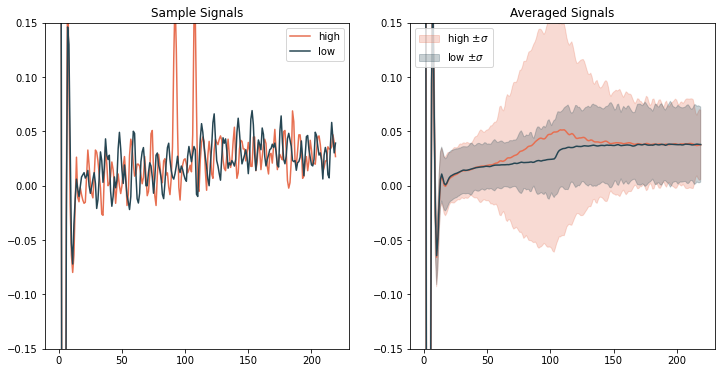
\includegraphics[width = \textwidth]{Figures/johann_first/sample.png}
    \caption{Comparison of the high and low pass signals. The left is an example of two read-outs (one high and one low respectively), while the right shows the averaged signals over the training set, the standard deviations are plotted as well.}
    \label{fig:samples}
\end{figure}



\begin{figure}[H]
    \centering
    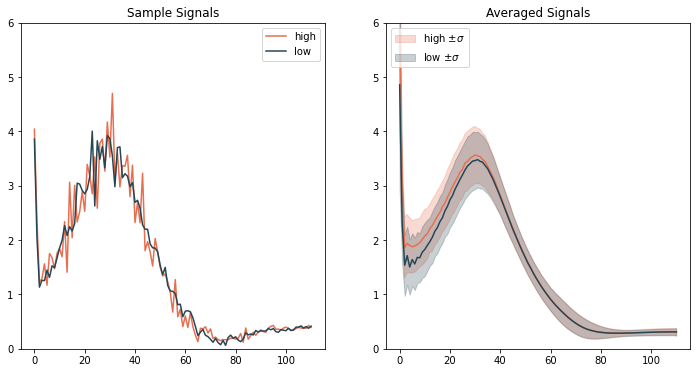
\includegraphics[width = 0.6 \textwidth]{Figures/johann_first/FFT_sample.png}
    \caption{Similar to Fig. \ref{fig:samples} but in a Fourier transformed space. Absolute value of frequencies are taken. The x-axis is just index and can be ignored. }
    \label{fig:samples_fft}
\end{figure}

\noindent
To do the classification, a few different methods were used. They are described in the following list. The ROC-curves for the methods are shown in Fig. \ref{fig:AUC_comparison} and the AUC and Accuracy is shown in Table \ref{tab:Metric Comparison}.


\begin{table}[h]
\centering
\caption{A comparison of the test-metrics for different methods, we tried in the classification process.}
\label{tab:Metric Comparison}
\begin{tabular}{lll}
Name                   & Accuracay & AUC   \\
peak\_height\_adjusted & \textit{0.836}     & \textit{0.875} \\
1D\_conv               & 0.855     & 0.906 \\
feed\_forward\_network & 0.796     & 0.87  \\
LSTM                   & \textbf{0.858}     & \textbf{0.912} \\
TCN                    & 0.798     & 0.891 \\
umap\_fft              & 0.804     & 0.867 \\
umap\_real\_time       & 0.746     & 0.805 \\
xgb\_real\_time        & 0.821     & 0.875
\end{tabular}
\end{table}

\begin{itemize}
    \item \textit{peak\_height\_adjusted} is a baseline model. Currently the readouts are made by looking for peaks in the read-out phase. This method takes the time signals in the interval from time-step 50 to 150 and looks for the maximum value. These values are now transformed using a Quantile Transformer to have a uniform distribution from 0 to 1, so it can be used as a probability and be compared to the other methods. Optimally the QuantileTransformer should be fit on training data and applied on the test set, but this was just fitted and transformed on test data as a first try.
    \item \textit{1D\_conv} This is 1d convolution neural network, which is build similar to the one used in \cite{Struck2020}. This model seems to perform very well and better than the baseline while being efficient to train.
    \item \textit{feed\_forward\_network}: This is a simple feed forward neural network inspired by the code send by Evert. It seems like different setups of the networks give around the same performance.
    \item \textit{LSTM}: Neural Network using LSTM layers. Since there is a lot of information in the individual time-steps all hidden-states are passed on to a new LSTM layer and afterwards flattened and passed to Dense layers to ultimately make the predictions. The LSTM networks are performing well and converges fast. However, LSTM networks pass one time-step at a time, so it is a lot slower than the other methods, and it is limited how much hyper-parameter tuning we can do on a laptop. Further performance gain could probably be found by using bidirectional layers.
    \item \textit{TCN}: Temporal Convolutional Networks emphasise on temporal correlation by only convoluting backwards in time. This does not compete with 1D-conv or LSTM.
    \item \textit{UMAP} The umaps are done by embedding similar to Fig. \ref{fig:UMAP_Classification} where the most dominant coordinate is used for classification. It would probably be clever to do a quantile transformation of the coordinate to obtain a more reliable accuracy, but umap is not performing as well as other methods so this is not done now.
    \item \textit{xgboost:} Just a straight-out-of-the-box method to have some baseline. With Fourier transformed data the result is slightly worse.
\end{itemize}



\begin{figure}[h]
    \centering
    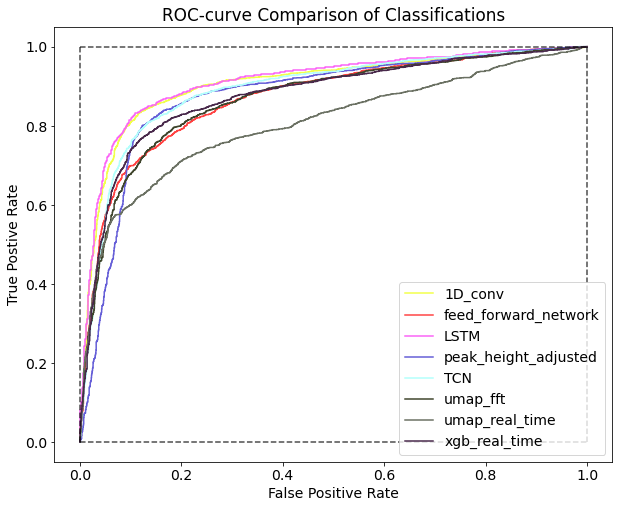
\includegraphics[width = 0.75 \textwidth]{Figures/johann_first/AUC_comparison.png}
    \caption{Comparison of the ROC curves for the different metods listed.}
    \label{fig:AUC_comparison}
\end{figure}

